\begin{XeClass}{FileSystem}
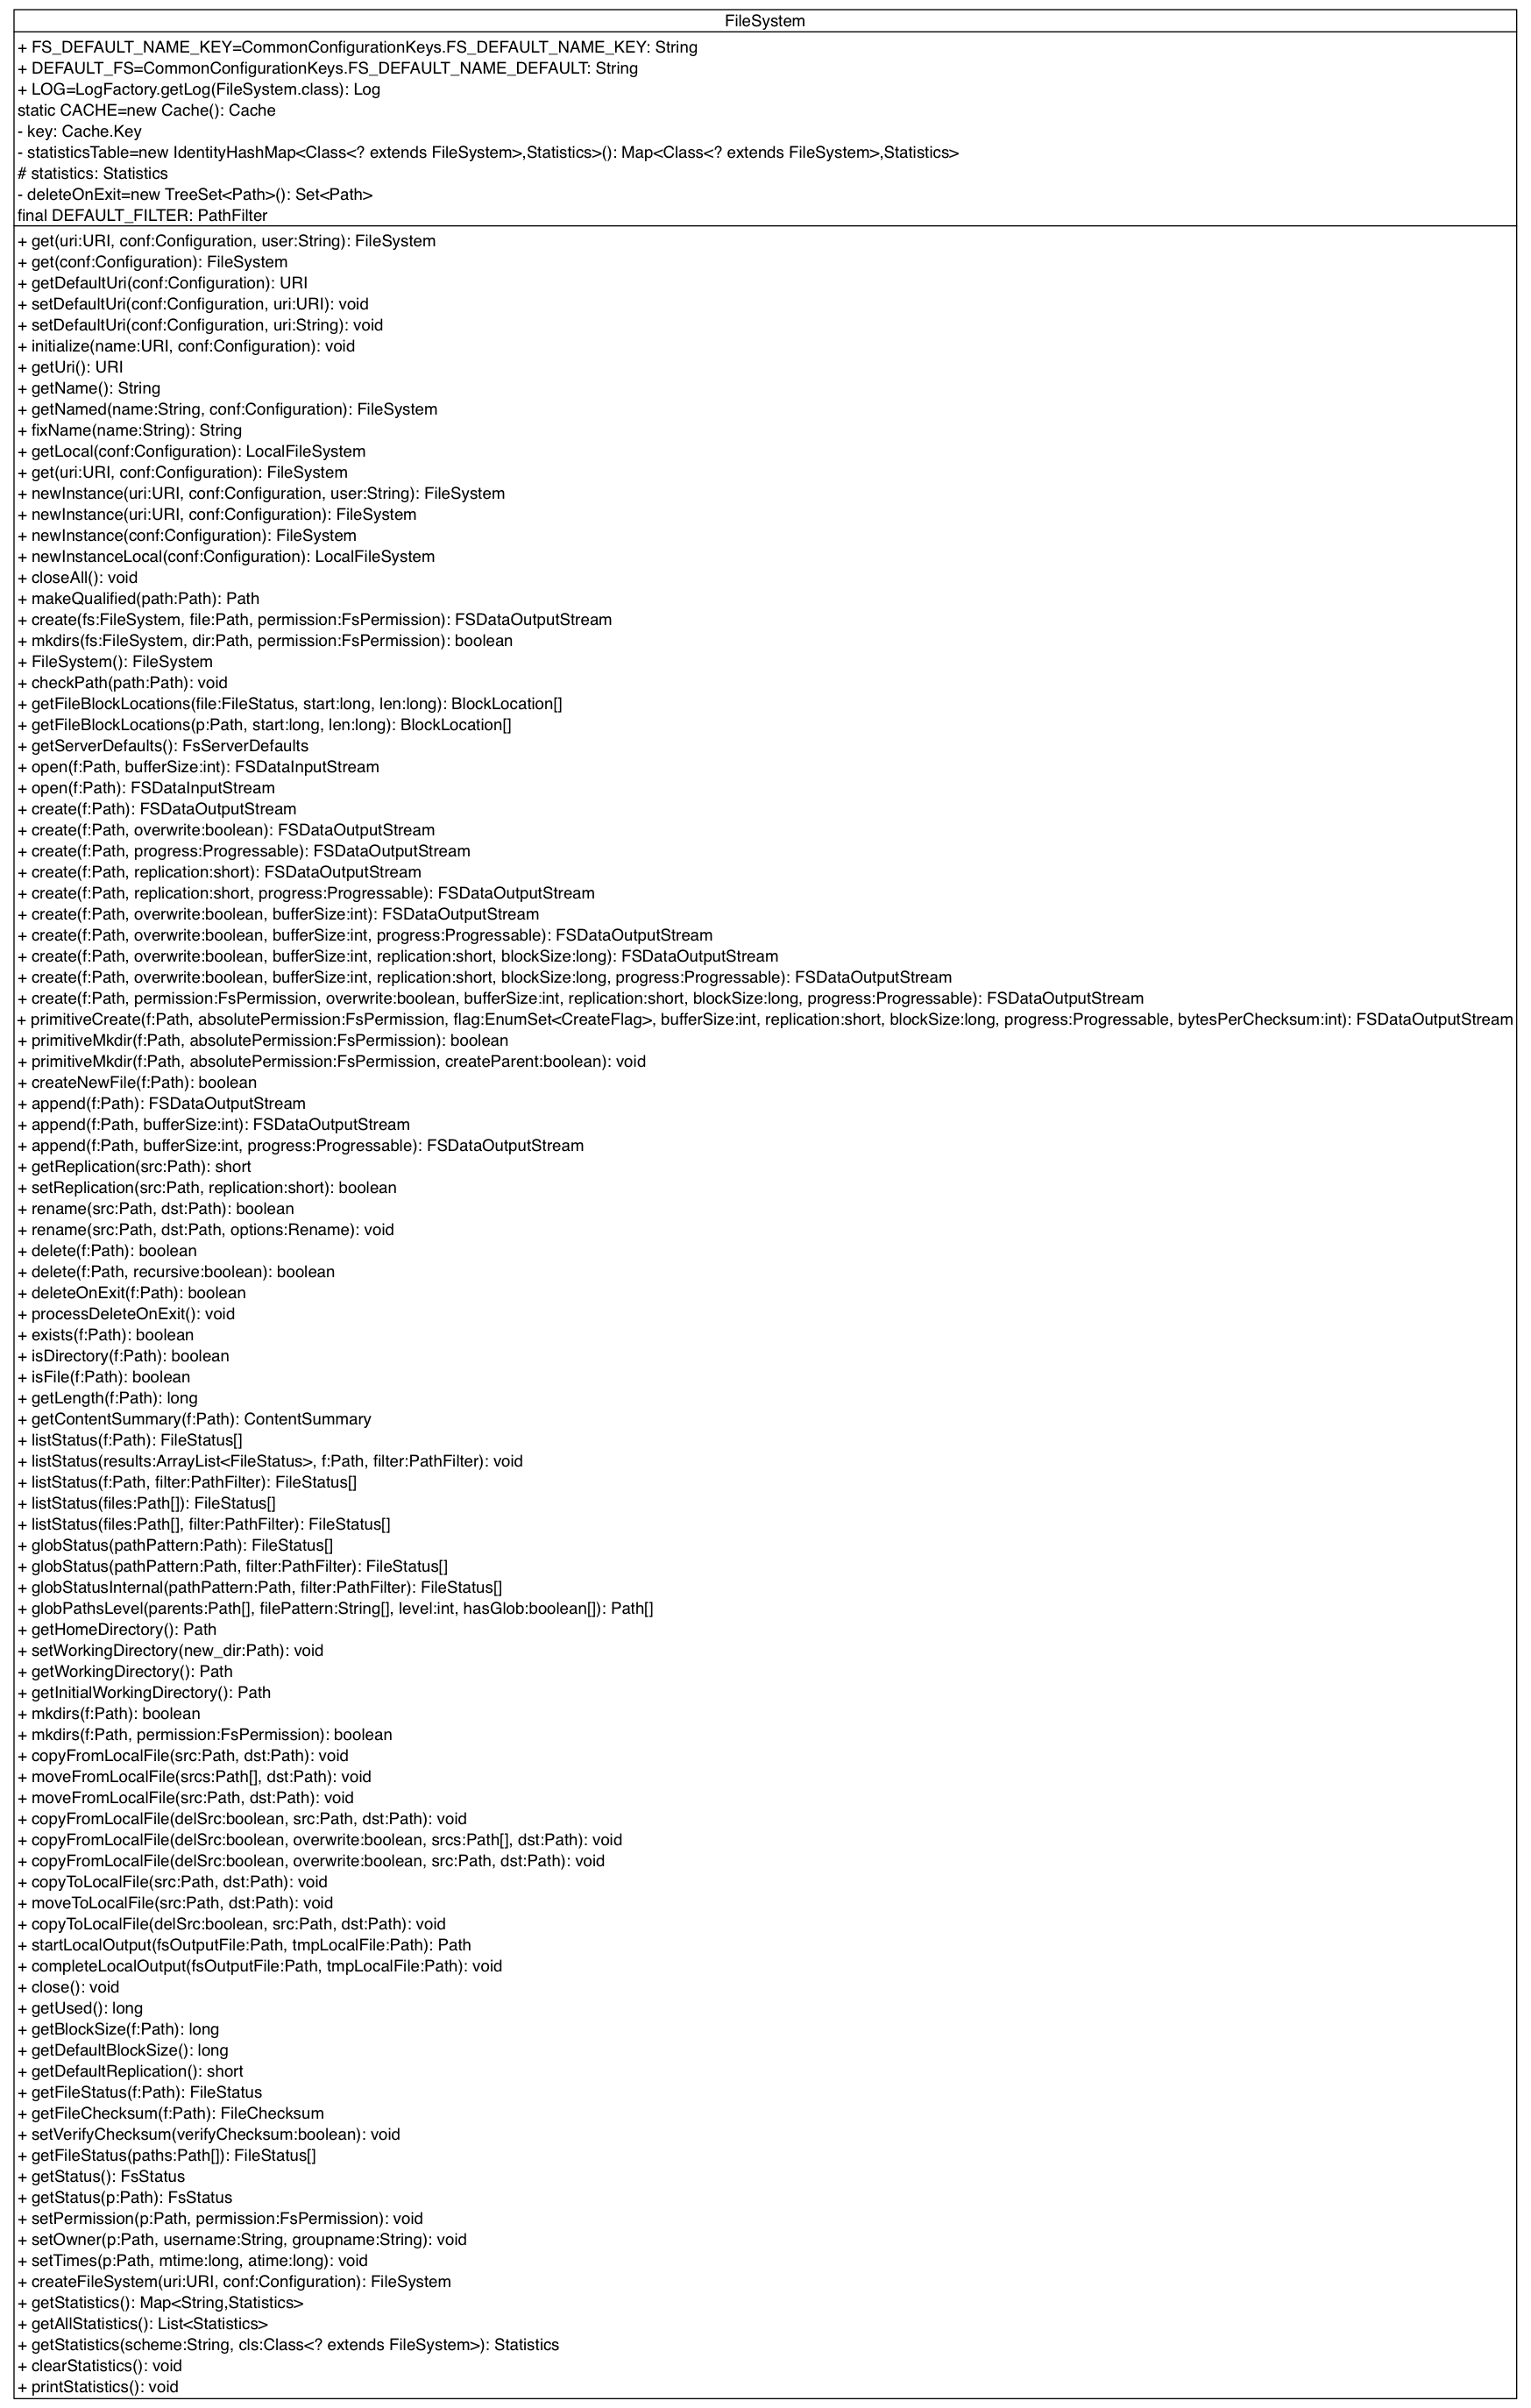
\includegraphics[width=10cm]{cdig/FileSystem.png}
     
 FileSystem(下简称FS)是一般的通用文件系统的抽象基类
 继承了Configured类,提供了访问配置文件的方法
 实现了Closeable接口,实现了关闭流的方法
 FS可以被实现为分布式的文件系统,如HDFS,亦或是一个本地的文件系统,
 所有具有访问HDFS的潜在可能的用户代码都应该被封装在一个FileSystem实例里。
 HDFS是一个对外表现如同单一磁盘的多机系统,
 它的容错能力和对大容量存储的支持使得HDFS尤为实用。
 
 1. 域:
 \begin{XeEnum}
 \item 文件系统的缓存
 \item 键
 \item 文件系统的子类与统计信息的映射
 \item 统计信息
 \item 缓存中文件路径的集合
 \end{XeEnum}
 
 2.内部类:
 \begin{XeEnum}
 \item Cache类:用来缓存文件系统
 \item ClientFinalizer类:JVM关闭是调用进行清理
 \item Key类:保存了与文件系统uri的信息,与文件系统对应
 \item Statistics:用来记录统计信息的类
 \end{XeEnum}
 
 3.方法:
 
 文件系统的关闭:
 \begin{XeEnum}
 \item closeAll()
 \item close()
 \end{XeEnum}
 
 文件系统的读取数据:
 \begin{quote}
 FSDataInputStream open(Path f, int bufferSize)
 \end{quote}
 
 文件系统的写入数据:
 \begin{quote}
 FSDataOutputStream create(Path f) \\
 FSDataOutputStream append(Path f) 
 \end{quote}
 
 重命名操作: \\
 boolean rename(Path src, Path dst)
 
 文件删除操作: \\
 boolean delete(Path f)
 
 文件或路径测试: \\
 \begin{XeEnum}
 \item boolean exists(Path f)
 \item boolean isDirectory(Path f)
 \item boolean isFile(Path f)
 \end{XeEnum}
 
 文件复制操作:
 \begin{XeEnum}
 \item copyFromLocalFile(Path src, Path dst)实现将文件从本地复制到其它路径
 \item copyToLocalFile(Path src, Path dst)负责将FS下的文件复制到本地
 \end{XeEnum}
 
 文件移动操作: \\
 \begin{XeEnum}
 \item moveFromLocalFile(Path[] srcs, Path dst)负责将本地文件移动到FS的其它位置
 \item moveToLocalFile(Path src, Path dst)将FS下的文件移动到本地
 \end{XeEnum}
  
 文件查询: \\
 \begin{XeEnum}
 \item FileStatus[] listStatus(Path f)
 \item FileStatus[] globStatus(Path pathPattern)
 \end{XeEnum}
  
 通配格式: \\
 interface PathFilter

    \begin{XeMethod}{\XePublic}{FileSystem}{get}
         
 通过URI、配置对象和用户来获取缓存中的一个文件系统对象
 具体过程为先判断用户字符串,若为空,则获取用户组信息的当前用户;
 若不为空,则创建远程用户。最后根据URI和配置对象返回文件系统对象

    \end{XeMethod}

    \begin{XeMethod}{\XePublic}{URI}{getDefaultUri}
         
 通过配置对象获取默认URI

    \end{XeMethod}

    \begin{XeMethod}{\XePublic}{void}{setDefaultUri}
         
 通过配置对象和URI设置默认URI

    \end{XeMethod}

    \begin{XeMethod}{\XePublic}{void}{initialize}
         
 通过URI和配置对象初始化,文件系统实例化后调用
 for this FileSystem

    \end{XeMethod}

    \begin{XeMethod}{\XePublic \\ \XeAbstract}{URI}{getUri}
         
 返回可以标示改文件系统的URI

    \end{XeMethod}

    \begin{XeMethod}{\XePrivate}{String}{fixName}
         
 为了向下兼容,更新旧格式的文件系统名字

    \end{XeMethod}

    \begin{XeMethod}{\XePublic}{LocalFileSystem}{getLocal}
         
 获取本地文件系统实例

    \end{XeMethod}

    \begin{XeMethod}{\XePublic}{FileSystem}{newInstance}
         
 Returns the FileSystem for this URI's scheme and authority and the
 passed user. Internally invokes \emph{.newInstance(URI,Configuration)}通过URI模式、权限和用户名返回文件系统实例

    \end{XeMethod}

    \begin{XeMethod}{\XePublic}{FileSystem}{newInstance}
         
 通过URI模式、权限和用户名返回文件系统实例。
 具体实现是通过读取配置文件中的\emph{fs.[scheme].Impl}对应
 的值。
 该方法总返回一个新的文件系统的值。

    \end{XeMethod}

    \begin{XeMethod}{\XePublic}{LocalFileSystem}{newInstanceLocal}
         
 获取一个唯一的本地文件系统实例

    \end{XeMethod}

    \begin{XeMethod}{\XePublic}{void}{closeAll}
         
 关闭所有缓存的文件系统实例。

    \end{XeMethod}

    \begin{XeMethod}{\XePublic}{Path}{makeQualified}
         
 该方法确认输入的路径可以确定一个文件系统

    \end{XeMethod}

    \begin{XeMethod}{\XePublic}{FSDataOutputStream}{create}
         
 通过提供的权限创建一个文件。
 通常的实现是使用两个RPC,虽然低效,但是是线程安全的。另一种可能是
 在设置中将umask设置为0,但这样就无法保证线程安全。

    \end{XeMethod}

    \begin{XeMethod}{\XePublic}{boolean}{mkdirs}
         
 通过提供的权限创建一个目录。

    \end{XeMethod}

    \begin{XeMethod}{\XeProtected}{void}{checkPath}
         
 检查路径是否属于该文件系统

    \end{XeMethod}

    \begin{XeMethod}{\XePublic}{BlockLocation[]}{getFileBlockLocations}
         
 返回一个文件的主机名、偏移量和分配的大小。
 对于一个不存在的文件,返回NULL。
 此方法对于DFS非常重要,DFSClient通过此方法来获取
 指定文件的Block所在的datanode。

    \end{XeMethod}

    \begin{XeMethod}{\XePublic}{FsServerDefaults}{getServerDefaults}
         
 返回默认服务器配置变量值

    \end{XeMethod}

    \begin{XeMethod}{\XePublic \\ \XeAbstract}{FSDataInputStream}{open}
         
 在指示的路径上打开一个文件系统的数据输入流

    \end{XeMethod}

    \begin{XeMethod}{\XePublic}{FSDataOutputStream}{create}
         
 在指定的路径上打开一个\emph{FSDataOutputStream},同时会打开一个
 进度报告。文件默认会被覆盖。

    \end{XeMethod}

    \begin{XeMethod}{\XePublic}{boolean}{createNewFile}
         
 在所给路径上创建一个全新的零长度的文件,如果文件已经存在,则会返回false。

    \end{XeMethod}

    \begin{XeMethod}{\XePublic}{FSDataOutputStream}{append}
         
 在一个存在文件上进行追加操作

    \end{XeMethod}

    \begin{XeMethod}{\XePublic}{short}{getReplication}
         
 获取文件系统的副本数量。

    \end{XeMethod}

    \begin{XeMethod}{\XePublic}{boolean}{setReplication}
         
 对一个存在的文件进行复制操作
 false if file does not exist or is a directory

    \end{XeMethod}

    \begin{XeMethod}{\XeProtected}{void}{rename}
         
 重命名一个文件。
 会在如下情形失败:
 - src是文件而dst是目录。
 - src是目录而dst是文件。
 - src或者dst的上级目录是文件。
 - 如果没有设置OVERWITE,且dst已经存在,则会失败。
 - 设置了OVERWRITE,但是dst是一个非的目录。
 注意,原子性的重命名操作取决于文件系统的实现,默认的实现是非原子的。

    \end{XeMethod}

    \begin{XeMethod}{\XePublic \\ \XeAbstract}{boolean}{delete}
         
 删除指定的文件

    \end{XeMethod}

    \begin{XeMethod}{\XePublic}{boolean}{deleteOnExit}
         
 标记一个在文件系统关闭的时候要被删除掉的路径。
 当JVM关闭的时候,所有的文件系统对象都会被自动关闭,
 那么所有被标记的路径都会被删除掉。

    \end{XeMethod}

    \begin{XeMethod}{\XeProtected}{void}{processDeleteOnExit}
         
 退出时进行删除操作。该方法会递归删除所有指定路径的文件。

    \end{XeMethod}

    \begin{XeMethod}{\XePublic}{boolean}{exists}
         
 检查路径是否存在

    \end{XeMethod}

    \begin{XeMethod}{\XePublic}{boolean}{isDirectory}
         
 判断路径是否为目录.

    \end{XeMethod}

    \begin{XeMethod}{\XePublic}{boolean}{isFile}
         
 判断路径是否为常规文件

    \end{XeMethod}

    \begin{XeMethod}{\XePublic}{long}{getLength}
         
 返回文件的字节数

    \end{XeMethod}

    \begin{XeMethod}{\XePublic}{ContentSummary}{getContentSummary}
         
 获取文件的内容总和,包括长度的总和、文件数量的总和
 和文件目录的总和。

    \end{XeMethod}

    \begin{XeMethod}{\XePublic \\ \XeAbstract}{FileStatus[]}{listStatus}
         
 列出指定目录下的所有文件的\emph{FileStatus}对象
 IOException see specific implementation

    \end{XeMethod}

    \begin{XeMethod}{\XePublic}{FileStatus[]}{listStatus}
         
 根据用户提供的路径过滤,列出查找到的文件的状态
 after applying the filter
 IOException see specific implementation

    \end{XeMethod}

    \begin{XeMethod}{\XePublic}{FileStatus[]}{globStatus}
         
 返回匹配路径模式并且满足用户提供的路径过滤的文件状态对象数组,

    \end{XeMethod}

    \begin{XeMethod}{\XePublic}{Path}{getHomeDirectory}
         
 返回当前用户在这个文件系统中的home目录
 默认返回"/user/$USER/"

    \end{XeMethod}

    \begin{XeMethod}{\XePublic \\ \XeAbstract}{void}{setWorkingDirectory}
         
 设置工作目录

    \end{XeMethod}

    \begin{XeMethod}{\XePublic \\ \XeAbstract}{Path}{getWorkingDirectory}
         
 返回工作目录
 Get the current working directory for the given file system

    \end{XeMethod}

    \begin{XeMethod}{\XeProtected}{Path}{getInitialWorkingDirectory}
         
 获取初始的工作目录.
 is returned; else a null is returned.

    \end{XeMethod}

    \begin{XeMethod}{\XePublic \\ \XeAbstract}{boolean}{mkdirs}
         
 根据路径和权限创建目录,功能上类似\emph{mkdir -p}

    \end{XeMethod}

    \begin{XeMethod}{\XePublic}{void}{copyFromLocalFile}
         
 将本地文件复制到该\emph{FileSystem}

    \end{XeMethod}

    \begin{XeMethod}{\XePublic}{void}{moveFromLocalFile}
         
 将本地文件移动到该\emph{FileSystem},源文件在被移动后会被删除。

    \end{XeMethod}

    \begin{XeMethod}{\XePublic}{void}{copyToLocalFile}
         
 将\emph{FileSystem}中的文件复制到本地文件系统,源文件在被移动后会被删除。

    \end{XeMethod}

    \begin{XeMethod}{\XePublic}{void}{moveToLocalFile}
         
 将\emph{FileSystem}中的文件移动到本地文件系统,源文件在被移动后会被删除。

    \end{XeMethod}

    \begin{XeMethod}{\XePublic}{Path}{startLocalOutput}
         
 返回一个本地文件,用户可以向此文件进行输出,而输出内容则会同步到
 目标文件系统

    \end{XeMethod}

    \begin{XeMethod}{\XePublic}{void}{completeLocalOutput}
         
 Called when we're all done writing to the target.  A local FS will
 do nothing, because we've written to exactly the right place.  A remote
 FS will copy the contents of tmpLocalFile to the correct target at
 fsOutputFile.
 完成本地文件输出。对于本地文件系统,此操作无用。但是对于远程文件系统,此操作会将
 tmpLocalFile拷贝到远程系统。

    \end{XeMethod}

    \begin{XeMethod}{\XePublic}{void}{close}
         
 关闭此文件系统。

    \end{XeMethod}

    \begin{XeMethod}{\XePublic}{long}{getUsed}
         
 返回此文件系统的所有文件的大小。

    \end{XeMethod}

    \begin{XeMethod}{\XePublic}{long}{getBlockSize}
         
 获取指定文件大小

    \end{XeMethod}

    \begin{XeMethod}{\XePublic}{long}{getDefaultBlockSize}
         
 获得默认的块大小。

    \end{XeMethod}

    \begin{XeMethod}{\XePublic}{short}{getDefaultReplication}
         
 Get the default replication.
 获得默认的文件副本数量。

    \end{XeMethod}

    \begin{XeMethod}{\XePublic \\ \XeAbstract}{FileStatus}{getFileStatus}
         
 给定目录的\emph{FileStatus}
 IOException see specific implementation

    \end{XeMethod}

    \begin{XeMethod}{\XePublic}{FileChecksum}{getFileChecksum}
         
 获得文件的校验和

    \end{XeMethod}

    \begin{XeMethod}{\XePublic}{void}{setVerifyChecksum}
         
 设置是否确认检验和的布尔标识

    \end{XeMethod}

    \begin{XeMethod}{\XePublic}{FsStatus}{getStatus}
         
 该方法返回一个指定路径所在的描述文件系统的已用量和容量的状态对象。
 the default partition.

    \end{XeMethod}

    \begin{XeMethod}{\XePublic}{void}{setPermission}
         
 设置路径的权限
 Set permission of a path.

    \end{XeMethod}

    \begin{XeMethod}{\XePublic}{void}{setOwner}
         
 设置路径的拥有者

    \end{XeMethod}

    \begin{XeMethod}{\XePublic}{void}{setTimes}
         
 设置文件的访问时间
 The number of milliseconds since Jan 1, 1970.
 A value of -1 means that this call should not set modification time.
 The number of milliseconds since Jan 1, 1970.
 A value of -1 means that this call should not set access time.

    \end{XeMethod}

    \begin{XeMethod}{\XePublic \\ \XeSync}{Map<String,Statistics>}{getStatistics}
         
 获取一个Map对象,该对象键为文件的scheme,值为统计对象。

    \end{XeMethod}

    \begin{XeMethod}{\XePublic \\ \XeSync}{List<Statistics>}{getAllStatistics}
         
 返回所有文件系统的统计对象。

    \end{XeMethod}

    \begin{XeMethod}{\XePublic \\ \XeSync}{Statistics}{getStatistics}
         
 获取指定文件系统的统计对象。

    \end{XeMethod}


    \begin{XeInnerClass}{Cache}
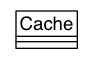
\includegraphics[width=10cm]{cdig/Cache.png}
         
 缓存文件系统对象的静态内部类
 1.主要记录了Key和文件系统的映射,以及Key的集合
 Key是Cache的内部类
 主要记录了模式信息,授权信息以及用户组信息
 2.其主要方法包括获取、删除、关闭Key所对应的文件系统实例

        \begin{XeInnerClass}{ClientFinalizer}
\includegraphics[width=10cm]{cdig/ClientFinalizer.png}
             
 ClientFinalizer类继承了Thread类
 当Java虚拟机停止运行时,该线程才会启动
 调用run进关闭清理工作

        \end{XeInnerClass}
        \begin{XeInnerClass}{Key}
\includegraphics[width=10cm]{cdig/Key.png}
             
 FileSystem.Cache.Key

        \end{XeInnerClass}
    \end{XeInnerClass}
    \begin{XeInnerClass}{Statistics}
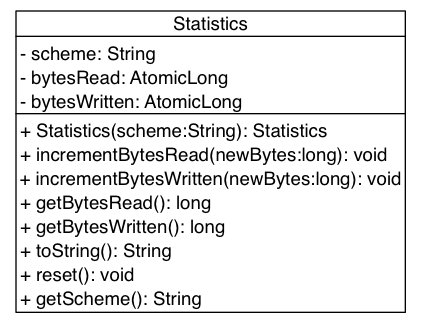
\includegraphics[width=10cm]{cdig/Statistics.png}
         
 统计信息——静态内部类
 主要包含了URI的模式信息,被用于AbstractFileSystem和link FileSystem
 URI格式是scheme://authority/path
 对HDFS文件系统,scheme是hdfs;对本地文件系统,scheme是file
 该类包含了对读写的字节数、读取的操作次数内容进行的记录

    \end{XeInnerClass}
\end{XeClass}
